\documentclass[beamer]{standalone}
\usepackage{circuitikz}
\begin{document}

\title[Electronics 1]{Operational amplifiers}

\begin{frame} 
  \titlepage
  \begin{figure}
  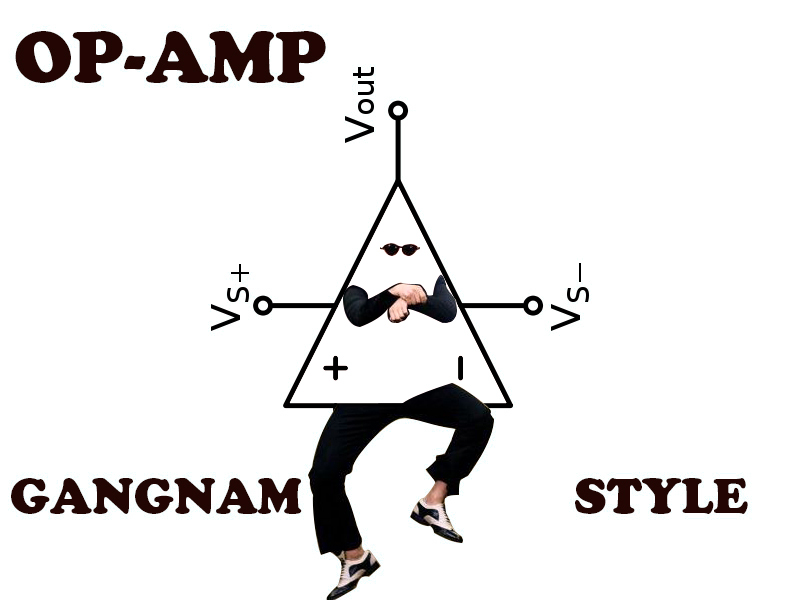
\includegraphics[height=0.4\textheight]{./pics/op_amp_gangnam_style_transparent.jpg}
  \end{figure}
\end{frame}

\section{Op-amps introduction}
\begin{frame}{Operational amplifiers (Op-Amp)}
 In the previous lecture we designed the AC inverting amplifier with transistors.  In the lab we made the amplification as large as we could by using a by-pass capacitor.
 \begin{figure}
  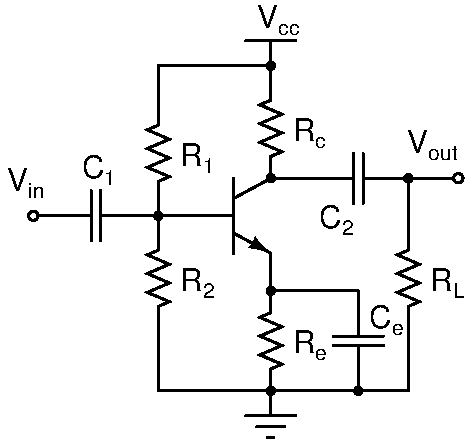
\includegraphics[height=0.45\textheight]{./schematics/npn_ac_common_emitter_amplifier_with_ac_boost}
  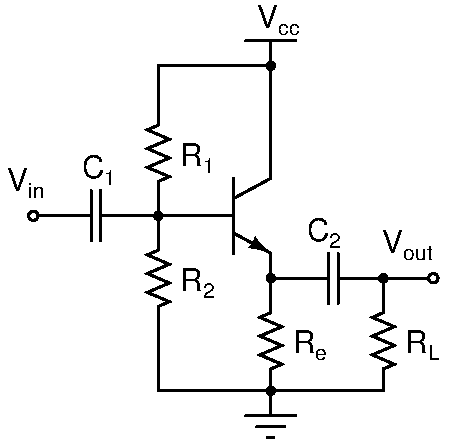
\includegraphics[height=0.45\textheight]{./schematics/npn_ac_emitter_follower}
\end{figure}
 With this amplifier even a small input voltage (and nearly zero input current) could lead to \emph{railed output}: the output is constant at $V_{cc} = 15$\,V or $V_{ee} = 0$\,V.  With emitter-follower we can make output impedance very small.
\end{frame}

\begin{frame}
\frametitle{Operational amplifiers (Op-Amp)}
\begin{figure}
	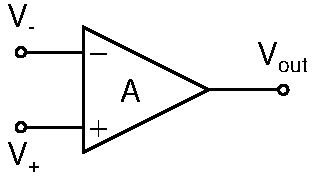
\includegraphics[width=0.30\textwidth]{./schematics/opamp.pdf}
\end{figure}
\begin{itemize}
	\item $V_{out}=A (V_+ - V_-)$ thus sometimes called differential
		amplifiers
	\item $A$ is open loop gain
		\begin{itemize}
			\item $A$ is frequency dependent
			\item $A=10^5 \dots 10^6$ at DC
			\item $A \to 0$ at high frequency (roll off)\\
				this limits operational bandwidth (typically in MHz \dots GHz range)
		\end{itemize}
	\item input impedances are high $10^6 \dots 10^{14}$~$\Omega$
	\item output impedances are low $0.1 \dots 10$~$\Omega$
		\begin{itemize}
			\item \alert{however output current usually limited to 10 mA}
		\end{itemize}
	\item {\bf it is super easy to design with them}
\end{itemize}
\end{frame}

\begin{frame}
\frametitle{If Op-Amps are so great why did we learn transistors?}
\vskip -.2in
\begin{columns}[t]
	\begin{column}{.45\textwidth}
		\begin{itemize}
			\item sometimes one transistor is enough and op-amps are more expensive
			\item op-amps are made of transistors so to understand their limits we
				need to know how transistors behave
			\item op-amps require bipolar power supply
			\item remember that op-amps cannot source a lot of current/power while
				transistors can (recall our transistor  controlled switch for a
				bulb)
		\end{itemize}
	\end{column}
	\begin{column}{.55\textwidth}

		\vskip .2in
		LM741 (introduced in 1968) internal schematic
		\begin{figure}
			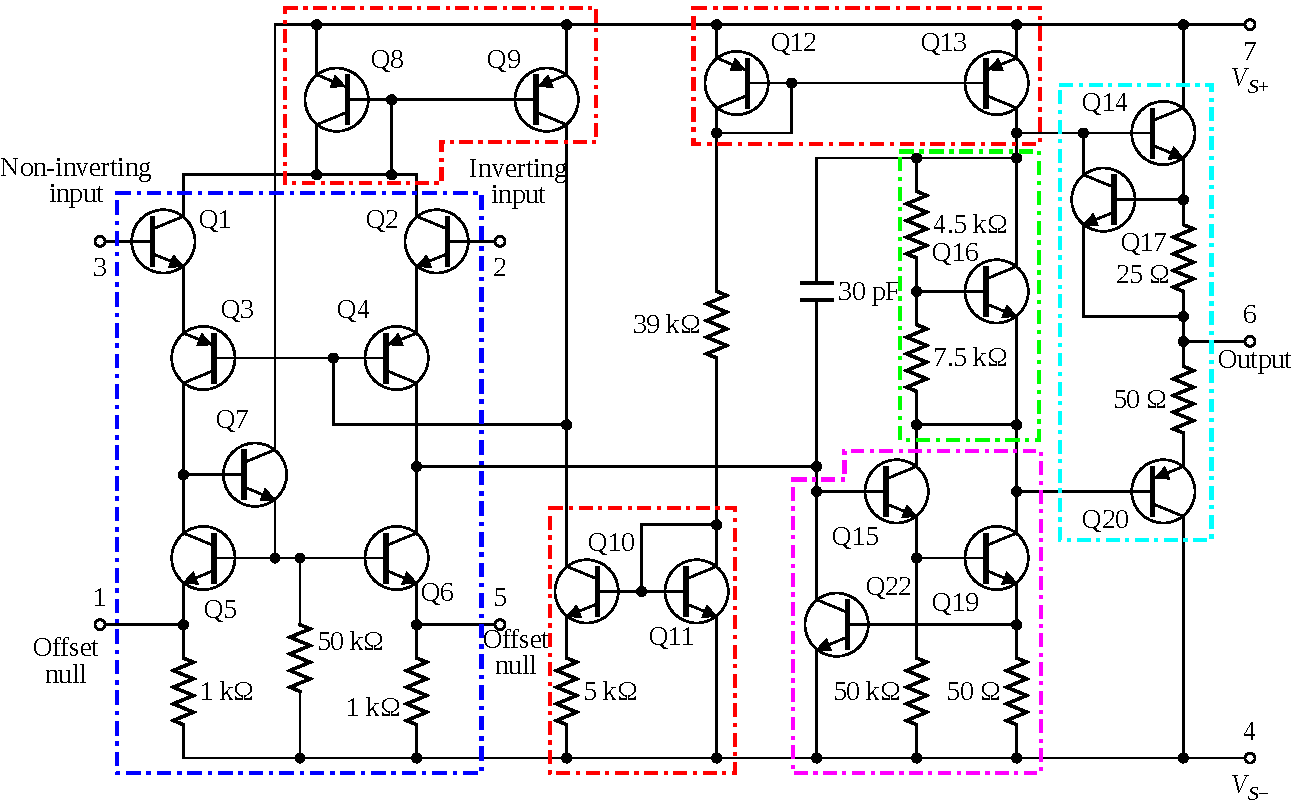
\includegraphics[width=1.00\columnwidth]{./pics/OpAmpTransistorLevel_Colored_Labeled}
		\end{figure}
		So, combine op-amps and transistors for a power circuits. Otherwise do your
		circuit with  op-amps.
		
	\end{column}
\end{columns}
\end{frame}
	

\section{Very bad amplifier}
\begin{frame}
\frametitle{Very very bad amplifier !!!}
\begin{figure}
	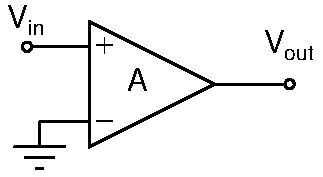
\includegraphics[width=0.30\textwidth]{./schematics/very_bad_amplifier.pdf}
\end{figure}

\begin{block}{Gain}
\begin{equation*}
	V_{out}=A V_{in}
\end{equation*}
But $A$ depends on everything
\begin{itemize}
	\item temperature
	\item power supply voltage
	\item input voltage
	\item frequency
	\item \dots and so on
\end{itemize}
\end{block}
\end{frame}

\section{Non-inverting amplifier}
\begin{frame}
\frametitle{Follower or Buffer}
\begin{figure}
	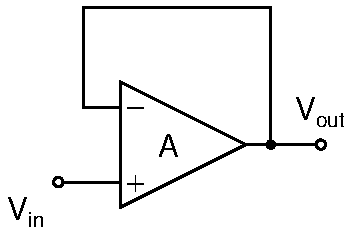
\includegraphics[width=0.30\textwidth]{./schematics/buffer.pdf}
\end{figure}
\begin{equation*}
	V_{out}=\frac{A}{A+1} V_{in}
\end{equation*}
\begin{block}{Gain  and impedances of ideal Op-Amp ($A \gg 1$)}
\begin{equation*}
	G_{ideal}=1
\end{equation*}
\begin{equation*}
	Z_{in}=\infty, Z_{out}=0
\end{equation*}
\end{block}
\alert{notice that with negative feedback $V_{+} \approx V_-$}
\end{frame}

\begin{frame}
\frametitle{Non-inverting amplifier}
\begin{figure}
	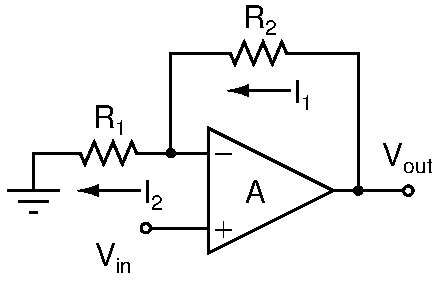
\includegraphics[width=0.30\textwidth]{./schematics/noninv_ampl.pdf}
\end{figure}
\begin{equation*}
	V_{out}=\left( 1+\frac{R_2}{R1} \right) V_{in}
	\frac{A}{A+(1+\frac{R_2}{R_1})}
\end{equation*}

\begin{block}{Gain  and impedances of ideal Op-Amp ($A \gg 1$)}
\begin{equation*}
	G_{ideal}=1+\frac{R_2}{R_1} 
\end{equation*}
\begin{equation*}
	Z_{in}=\infty, Z_{out}=0
\end{equation*}
\end{block}
\alert{notice that with negative feedback $V_{+} \approx V_-$}
\end{frame}
	
\section{Op-amps golden rules}
\begin{frame}
\frametitle{Op-amps golden rules}
If \alert{negative feedback is applied} and \alert{$A(f) \gg 1$} (open
circuit gain  at the frequency of interest)
\begin{itemize}
	\item there is no current into the inputs
	\item $V_- = V_+$
\end{itemize}
\begin{block}{Gain of non ideal Op-Amp ($A \not\gg 1$)}
	\[ G=G_{ideal} || A 
	=	\frac{G_{ideal} A}{G_{ideal} + A}\]
\end{block}
\end{frame}

\section{Inverting amplifier}
\begin{frame}
\frametitle{Inverting amplifier}
\begin{figure}
	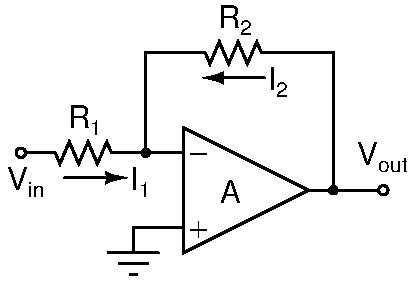
\includegraphics[width=0.30\textwidth]{./schematics/inv_ampl.pdf}
\end{figure}

\begin{block}{Gain  and impedances of ideal Op-Amp ($A \gg 1$)}
\begin{equation*}
	G_{ideal}=-\frac{R_2}{R_1}
\end{equation*}
\begin{equation*}
	Z_{in}=R_1, Z_{out}=0
\end{equation*}
\end{block}
\alert{notice that with negative feedback $V_{+} \approx V_-$}
\end{frame}
	
\section{Summing inverting amplifier}
\begin{frame}
\frametitle{Summing inverting amplifier}
\begin{figure}
	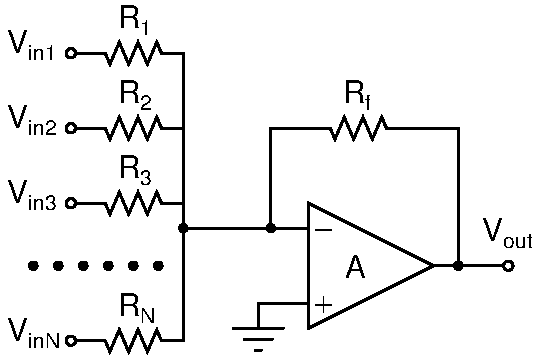
\includegraphics[width=0.30\textwidth]{./schematics/summing_inv_ampl.pdf}
\end{figure}

\begin{block}{for ideal Op-Amp ($A \gg 1$)}
\begin{equation*}
	V_{out}= -\left( 
	\frac{V_{in1}}{R_1} 
	+  \frac{V_{in2}}{R_2}
	+\frac{V_{in3}}{R_3} 
	+ \cdots 
	+ \frac{V_{inN}}{R_N} \right) R_f
\end{equation*}
\begin{equation*}
	Z_{inN}=R_N, Z_{out}=0
\end{equation*}
\end{block}
\end{frame}
	
\section{Differential amplifier}
\begin{frame}
\frametitle{Differential amplifier}
\begin{figure}
	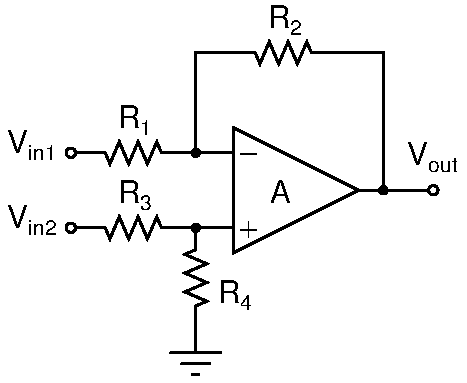
\includegraphics[width=0.30\textwidth]{./schematics/differential_ampl.pdf}
\end{figure}

\begin{block}{for ideal Op-Amp ($A \gg 1$)}
\begin{equation*}
	V_{out}= 
	 \frac{R_4}{R_1} \frac{R_1+R_2}{R_3+R_4} V_{in2}- \frac{R_2}{R_1}V_{in1}
\end{equation*}
\begin{equation*}
	 Z_{out}=0
\end{equation*}
\end{block}
\end{frame}

\end{document}
